\section{Node.js}
Node.js is a JavaScript running environment (runtime).In fact it is encapsulate Google V8 engine.The speed of V8 engine execute JavaScript is very fast, performance is very good. Node. Js optimize some special cases, provides alternative API, makes the V8 running better in the browser environment. 
It also is a platform which based on Chrome JavaScript, be used to build network Application with fast response speed and expand easily.\\
\\
Working principle see graph \ref{fig:bb cubed graph}:
\begin{figure}[h]
	\centering
	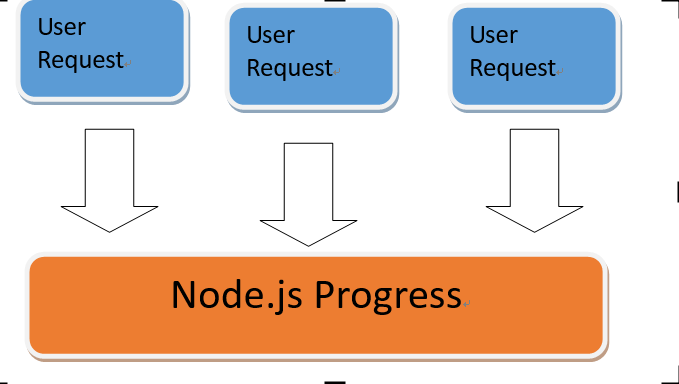
\includegraphics[scale=0.5]{a.png}
	\caption{Shopping Cary Mini State window}
	\label{fig:bb cubed graph}
\end{figure}
\\
\section{Database}	 
MongoDB was used to store all the data in shopping system include users' information and items' detail such as price, name, id and color.\\
MongoDB is classified as a NoSQL database and also is a cross-platform document-oriented database. \cite{2}
There have some features let me choose MongoDB:
Support JSON-file (MongoDB calls the format BSON), it let me import data easy and fast than SQL or MySQL. It can import JSON file or CSV use a line of code, see code put below.\\
Setting code : /bin  mongoimport –d cms –c –type csv –file c.csv -h localhost -port 11111 –upsert -f name

MongoDB have 6 main data type:\\
Number, String, Boolean, Array, Object, Null.

\section{JSON} \cite{11}
JSON (JavaScript Object Notation) is a lightweight data-interchange format. Sometimes JSON is an open-standard format that uses human-readable text to transmit data objects consisting of attribute–value pairs. It is the most common data format used for asynchronous browser/server communication (AJAJ), largely replacing XML which is used by AJAX.\\
\\
Exapmle of JSON file :

var jason = {


"age" : "24",


"hometown" : "Missoula, MT",


"gender" : "male"

};\\
\\
And it also can include the Emoji character U+1F602 (cryface) FACE WITH TEARS OF JOY in JSON:
\{ "face": "(cryface)" \} or\\ 
\{ "face": "\ uD83D \ uDE02" \}
\\
\section{Express.js}	
Express.js is a simple and flexible web application framework in Node.js, it’s not upgrade version of node.js but add a lot of powerful feature on web development.\\
Current Express.js Version: 2.14.7\\
\\
Install code: npm install express\\
var express = require('express');\\
\\
\section{Mongoose} \cite{10}
Firstly, I have used MongoDB self to operate Database, it generate many problems such as \\
Error: db object already connecting, open cannot be called multiple times.\\
I waste a lot of time to solve this problem, finally I find the problem is sometimes I refresh webpage too fast and the Database didn’t close will result in this problem.\\
There also have some others problem let me give up use mongodb self to control Db in Node.js.\\
I give a compare example below:\\
First step: npm install mongoose --save\\
var mongoose = require('mongoose');\\
mongoose.connect('mongodb://localhost/test');\\
Mongodb: every time operate DB need mongodb. Open (), and mongodb. Close () in the end. \\
\\
User.get = function get(username, callback) \{\\
	mongodb.open(function(err, db) {\\
		if (err) \{\\
			return callback(err);\\
		\}\\
		Read users collection\\ 
		db.collection('users', function(err, collection) \{\\
			if (err) \{\\
				mongodb.close();\\
				return callback(err);\\
			\}\\
			//find a file name is username in collection\\
			collection.findOne(\{name: username\}, function(err, doc) \{\\
				mongodb.close();\\
				if (doc) callback (err, doc);\\
				else callback (err, null);\\
			\});\\
		\});\\
	\});\\
\};\\
\\
Mongoose operate DB: Only need a few lines code\\
\\
User.get = function get(username, callback) \{\\
	users.findOne(\{name:username\}, function(err, doc)\{\\
		if (err) \{\\
			return callback(err, null);\\
		\}\\
		return callback(err, doc);\\
	\});\\
\};\\
\\
And paste some mongoose method below:\\
Create : \\
\\
DB.save(function (err) \{\\
	if (err) \\
	console.log('meow');\\
\});\\
Remove\\
\\
DB.remove(\{name:”ccc”\},function (err) \{\\
	if (err) // ...\\
	console.log('meow');\\
\});\\

Etc.



\section{Ajax}\cite{12}
Ajax (Asynchronous JavaScript and XML) is a very powerful technology that exchange a small amount of data in the back-end let website don’t need refresh of loading all data in the website again to update apart of website.\\
\\
Ajax module compare with traditional module\\
\\
Example of Ajax in Node.js, see graph \ref{fig:17 cubed graph}
\begin{figure}[h]
	\centering
	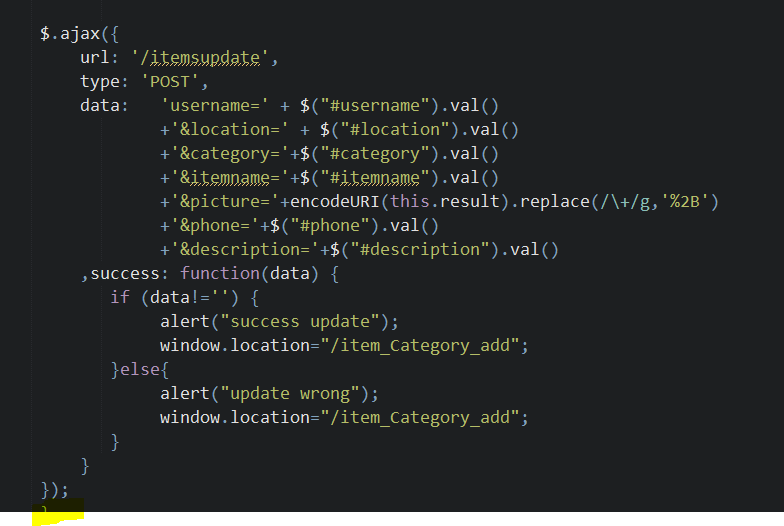
\includegraphics[scale=0.5]{5.png}
	\caption{Ajax}
	\label{fig:17 cubed graph}
\end{figure}
\\
\section{Crypto-js}	
This is a modular in npm that offer methods to encrypt and decrypt information.
Node using the OpenSSL library to realize its encryption technology, this is because the OpenSSL already is a widely used encryption algorithm.It includes similar MD5 or SHA - 1 algorithm, these algorithms you can use in your application.\\
\\
And crypto modular use Asymmetric encryption that refers to both sides in a different KEY encryption and decryption expressly, communication both sides have their own public KEY and private KEY.\\ 
Easy to understand, for example, we are assuming that communication both sides respectively is A and B. A, have KEY\_A1 KEY\_A2, including KEY\_A1 is a private key, KEY\_A2 is a public key, B has the KEY\_B1, KEY\_B2, including KEY\_B1 is B's private key, KEY\_B2 is B's public key. The characteristics of public key and private key is, after any of them a plaintext encrypted, can only use the other one was able to solve. That is to say after plaintext encrypted KEY\_A1, only can decrypt KEY\_A2, and vice versa.
\\
\subsection{Support Algorithms}
Crypto-js support many algorithms such as MD5, SHA-1, SHA-256, AES, Rabbit, MARC4, HMAC (HMAC-MD5, HMAC-SHA1, HMAC-SHA256), PBKDF2.
\\
\section{Session \cite{session}} 
In a web application user’s opinion, he opens a browser to access e-commerce site , log in and complete the shopping until you close your browser , this is a conversation . In web application developer’s mind, they need to create a data structure to store the user's information when a user login, this structure also called session. So we talk about session time to pay attention to context. The article talking about is based on the HTTP protocol to enhance the ability of the mechanism web application or a scheme , it does not refer to a specific dynamic page technology , and this ability is to keep the state and to be called to keep session.\\
Session have many advantages in different part such as security, property, convince.
And sometimes if we need session have long statement cycle, such as many web sites have a password the function of the automatic login within two weeks. Based on this requirement, the session must be looking for memory storage load, the database can provide the perfect solution. Here, I choose MongoDB as database, as a NoSQL database, data object database - collection - the basis of it the document object model is very intuitive and easy to understand, in view of the node.Js also provides rich drives and API. Express framework provides for directing a middleware: connect - mongo, we just at the time of mount session in the options to mongo parameters, program is running, express the app will automatically managing the session storage for us, update, and delete.\\
\\
Install Session: npm install express-session \\
And install a middleware: npm install connect-mongodb \\
\\
\section{Nodemailer}	 
This is a modular in node.js which can send email automatically. It’s very helpful in my shopping website I can send email to consumer when he or she successed register a account. And also send email to them when they finish an order.\\
\\
Install code: npm install nodemailer –save\\
\section{Autocomplete.js}\cite{13}
This is a JQuery technic, it can fill the search box automatically realize the function like Google search.\\
\\
The example picture \ref{fig:16 cubed graph} show below: 
\\
\begin{figure}[h]
	\centering
	
\includegraphics[scale=0.5]{39.png}
	\caption{Actocomplete fill}
	\label{fig:16 cubed graph}
\end{figure}
\\
License: \\
Ajax Autocomplete for jQuery is freely distributable under the terms of an MIT-style license.\\
Copyright notice and permission notice shall be included in all copies or substantial portions of the Software.\\
\\
\section{PayPal sandbox}
\\
PayPal Sandbox environment is an independent Environment and in a Sandbox environment does not involve actual money transactions. Its purpose to provide developers and integration environment, The Sandbox allows you to have the opportunity to before transplantation applications to a true PayPal to you the whole process of integration testing, avoid deployed to the possible problem in real environment.
\\
\section{Base64}
Base64 is a group of similar binary-to-text encoding schemes that represent binary data in an ASCII string format by translating it into a radix-64 representation. The term Base64 originates from a specific MIME content transfer encoding.\\
\\
The Node has a binary Buffer, the pseudo class provides a series processing of binary data API, simplifies the need to deal with the task of binary data. The length of the buffer is determined by the length of the byte data, and you can random set and get bytes of data in the buffer.\\
\\
var utf8String = 'my string';\\
var buf = new Buffer(utf8String);\\
var base64String = buf.toString('base64')\\
\\
\section{date-utils}
\\
Date-utils is a package in npm. In Nodejs get current system time is hard then other programming languages and Node provide a class to display time.\\
\\
install : npm install date-utils\\
require('date-utils');\\
var dt = new Date();\\
console.log(dt.toFormat("YYYY-MM-DD HH24:MI:SS"));\\
\\
\section{Regular Expression\cite{18}}
In theoretical computer science and formal language theory, a regular expression (sometimes called a rational expression) is a sequence of characters that define a search pattern, mainly for use in pattern matching with strings, or string matching, i.e. "find and replace"-like operations. The concept arose in the 1950s, when the American mathematician Stephen Kleene formalized the description of a regular language, and came into common use with the Unix text processing utilities ed, an editor, and grep, a filter.
I use Regular Expression to match some word that on search function which can get more similar words. And it also helpful on MondoDB to search data. 